\documentclass[a4paper, 11pt, nofootinbib]{article}

\setcounter{tocdepth}{3}
\setcounter{secnumdepth}{3}
\usepackage{amsmath}
\usepackage{comment} % enables the use of multi-line comments (\ifx \fi) 
\usepackage{lipsum} %This package just generates Lorem Ipsum filler text. 
\usepackage{fullpage} % changes the margin
\usepackage[utf8]{inputenc}
\usepackage{gensymb}
\usepackage{graphicx}
\usepackage{booktabs}% http://ctan.org/pkg/booktabs
\usepackage{makecell}
\usepackage{tabularx}
\usepackage[table]{xcolor}
\usepackage{array}
\usepackage{wrapfig}
\usepackage{subcaption}
\usepackage{csquotes}
\usepackage{lscape}
\usepackage{afterpage}
\usepackage{geometry}
\usepackage{listings}
\usepackage{xcolor}
\usepackage{ulem}
\usepackage{caption}

\definecolor{dkgreen}{rgb}{0,0.6,0}
\definecolor{gray}{rgb}{0.5,0.5,0.5}
\definecolor{mauve}{rgb}{0.58,0,0.82}

\lstset{frame=tb,
	language=Java,
	aboveskip=3mm,
	belowskip=3mm,
	showstringspaces=false,
	columns=flexible,
	basicstyle={\small\ttfamily},
	numbers=none,
	numberstyle=\tiny\color{gray},
	keywordstyle=\color{blue},
	commentstyle=\color{dkgreen},
	stringstyle=\color{mauve},
	breaklines=true,
	breakatwhitespace=true,
	tabsize=3
}

\geometry{a4paper, margin=1in}

\renewcommand{\figurename}{Abb.}
\newcommand{\code}[1]{\texttt{#1}}
\renewcommand{\contentsname}{Inhalt}
\renewcommand{\listfigurename}{Abbildungsverzeichnis}

\begin{document}
\title{Zusammenfassung Information Security FS2018}
\author{Alex Neher}
\maketitle

\tableofcontents
\newpage
\listoffigures
\newpage

\graphicspath{{./Pictures/}}

\section{Teil Pouly}
\subsection{Nach welchen Kriterien lassen sich Hacker und ihre Opfer klassifizieren?}

\paragraph{Hacker}\mbox{}\\

\noindent • Hacktivisten\\
• Cyberterroristen\\
• Staatliche Organisationen\\
• Skript Kiddies\\
• Organisiertes Verbrechen\\
• Wissenschaftler / Krypto-Analytiker\\

\paragraph{Opfer}\mbox{}\\

\noindent • Einzelpersonen (gezielt)\\
• Einzelpersonen (zufaellig)\\
• Die grosse Masse (zufaellig)\\
• Organisationen / Firmen (gezielt)\\

\subsection{Wleche Angriffstrategien werden typischerweise gegen welche Opfer eingesetzt?}

\begin{itemize}
	\item Einzelpersonen (gezielt)
		\subitem Identitätsdiebstahl
		\subitem Informationsdiebstahl
		\subitem Diskreditierung
	\item Einzelpersonen (zufällig)
		\subitem Phishing
		\subitem Skimming
	\item Die grosse Masse (zufällig)
		\subitem Viren-Angriffe auf bestimmte Betriebssysteme
	\item Firmen und Organisationen (gezielt)
		\subitem DDoS
\end{itemize}

\subsection{Beschreiben Sie zwei unterschiedliche Geschäftsmodelle von Hacking Organisationen}
\begin{itemize}
	\item Erpressung
	\item DDoS As a Service
\end{itemize}

\subsection{Was versteht man unter Identitätsdiebstahl?}
1. Ein Hacker stielt das E-Mail Passwort seines Vorgesetzten.\\
2. Ein Hacker stielt das Login Passwort zum PC eines Mitarbeiters.\\
3. Ein Hacker stielt ein Facebook Passwort.\\

In den USA ist Identitaetsdiebstahl ein grosses Problem, weil es dort – anders
als in der Schweiz – mit der Sozialversicherungsnummer ein personenbezogenes
Merkmal gibt, das hinreichend ist, um Steuern zurueckzufordern und Kreditkar-
tenvertraege abzuschliessen. [...] Allein 2011 belief sich der finanzielle Schaden
infolge von Identitaetsdiebstahl auf 3.6 Mrd. USD. NZZ, 20.01.2014

\subsection{Beschreiben Sie mögliche Konsequenzen von Identitätsdiebstahl für die Opfer}
• Finanzielle Folgen (Bestellungen auf meinen Namen etc)\\
• Rechtliche Folgen (Kinderpornografie etc)\\
• Gesellschaftliche Folgen (Postings von meinem FB Account)\\

\newpage

\subsection{Analysieren Sie die Authentifikationsmethoden 1-4 auf Stärken und Schwächen}

\begin{figure}[htb]
	\centering
	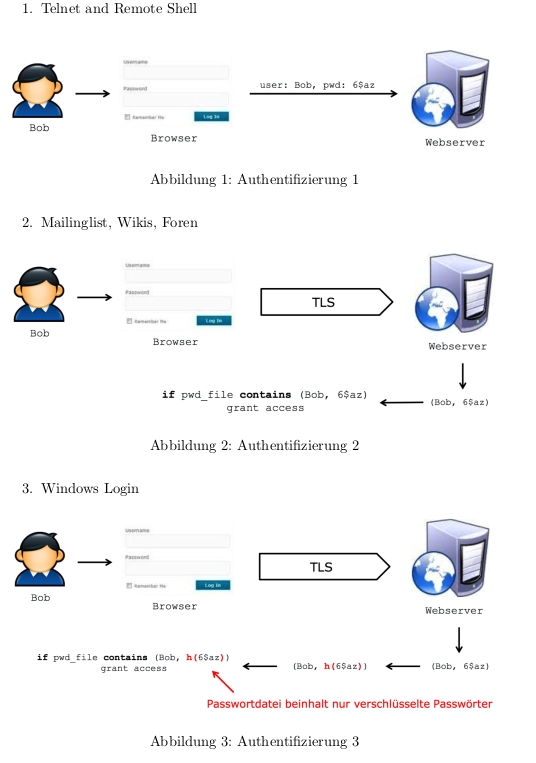
\includegraphics[keepaspectratio=true,height=27\baselineskip]{authentification.jpg}
\end{figure}
\begin{figure}[htb]
	\centering
	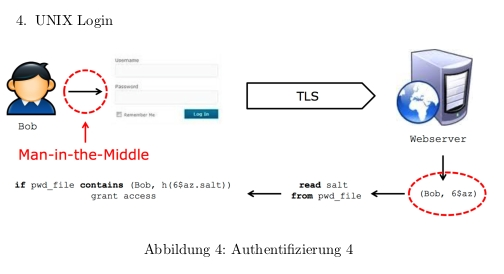
\includegraphics[keepaspectratio=true,height=9\baselineskip]{authentification_2.jpg}
\end{figure}

\newpage

\subsection{Wie schützen Betriebssysteme typischerweise unsere Identitäten und wie kann dieser Schutz mit Maschinenzugriff ausgehebelt werden?}
\paragraph{Windows}\mbox{}\\
Windows Betriebssysteme (seit NT) speichern Passwortinformationen in der Re-
gistry Datei Security Account Manager (SAM). Windows Kernel sichert SAM,
so dass Datei nicht kopiert werden kann.

So geht es trotzdem...
Dumping File Sectors directly from Disk using Logical Offsets $\rightarrow$ Cain\\
Wenn SysKey aktiviert ist, verschluesselt Windows die SAM Datei partiell.\\
Wenn SysKey aktiviert ist, holt bkhive den Schluessel aus der Registry.\\

\begin{figure}[htb]
	\centering
	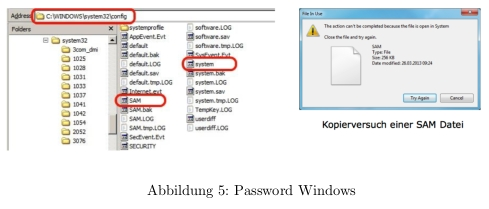
\includegraphics[keepaspectratio=true,height=12\baselineskip]{SAM_Windows.jpg}
\end{figure}

\paragraph{Linux}\mbox{}\\
Unix Betriebssysteme (seit 1990) speichern Passwortinformationen in Shadow
Dateien. Nur Superuser koennen diese Dateien lesen.

\begin{figure}[htb]
	\centering
	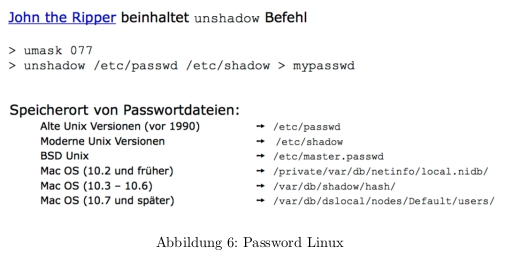
\includegraphics[keepaspectratio=true,height=12\baselineskip]{password_linux.jpg}
\end{figure}

\paragraph{Fazit}\mbox{}\\
• In Klartext gespeicherte (z.B. FileZilla) oder gecachte (z.B. Windows-
Domaenen Anmeldung) Passwoerter koennen mit Maschinenzugriff leicht
geklaut werden.\\
• Betriebssysteme schuetzen Passwortdateien, jedoch kann der Schutz leicht
umgangen werden.\\
• Anwendungsprogramme und Betriebssysteme verschluesseln Passwoerter
bevor sie in einer Passwortdatei abgelegt werden.\\

\subsection{WelcheAngriffsstrategien auf gestohlene Passwort-Hashes hat ein Hacker zur Verfügung?}

\begin{enumerate}
	\item Passwort-Hashfunktion knacken
	\item Brute-Force Attacke
		\subitem Alle möglichen Kombinationen werden systematisch durchprobiert
		\subitem Jedes mögliche Passwort wird verschlüsselt und in der Passwort-Datei gesucht
		\subitem Irgendeinmal wird jedes System so geknackt $\rightarrow$ Vollständige Methode
	\item Dictionary Attacke
		\subitem Nur Wörter aus einem vorgegebenen Wörterbuch werden durchprobiert
		\subitem Beruht auf der Annahme, dass sinnvolle Wörter als Passwort verwendet werden, oder dass das Passwort auf einem Algorithmus beruht (z.B. Palindrom)
		\subitem Knackt das System nur, falls sich das Passwort im Wörterbuch befindet $\rightarrow$ Unvollständige Methode
	\item Lookup Tabelle
		\subitem Wörterbuch mit Wort und dazugehörigem Hash
		\subitem Wörterbuch mit 1 Million Wörtern verlangt 1 Million Hashberechnungen
		\subitem Es muss nun nur noch nach dem Hashwert gesucht werden
		\subitem Es wird mehr Memory benötigt, dafür wird Zeit gespart
		\subitem Gleich wi<e Dictionary-Attack: Knackt nur Passwörter in der Tabelle $\rightarrow$ Unvollständige Methode
\end{enumerate}

\subsection{Sie können den Aufwand von Brute-Force Attacken vorausbereichnen}
Passwörter bestehen aus alphanumerischen Symbolen (a-z,A-Z,0-9) und 8 möglichen Zusatzzeichen ( 26 + 26 + 10 + 8 = 70 Zeichen). Das CMS Joomla verschlüsselt die Passwörter mit MD5. Angenommen, man verwendet die Software oclHashcat und 2 GPUs mit 880Mhz getaktet und 1250Mhz getaktete RAM. Die Benchmark zeigt 23083.9 M/s an $\rightarrow$ ca. $23 * 10^{9}$ Hashes/s

\paragraph{Passwort der Länge 7}\mbox{}\\
\begin{equation}
\dfrac{70^{7}  Hashes}{23*10^{9}   Hashes/sek} = 358sek = 5.96 Min \nonumber
\end{equation} 

\paragraph{Passwort der Länge 9}\mbox{}\\
\begin{equation}
\dfrac{70^{9}  Hashes}{23*10^{9}   Hashes/sek} = 1754504sek = 487.3h = 20.3 Tage \nonumber
\end{equation} 

\paragraph{Passwort der Länge 11}\mbox{}\\
\begin{equation}
\dfrac{70^{11}  Hashes}{23*10^{9}   Hashes/sek} = 8597072795sek  = 99503 TAge = 272.6 Jahre \nonumber
\end{equation} 

\subsection{Nennen Sie den Unterschied zwischen Dictionaries und Lookup-Tabellen}
Lookup-Tabellen sind vorgefertigte Tabellen, die einen Hashwert und das dazugehörige Klartext-Passwort enthalten. Die Hashes sind bereits berechnet. Man muss nur noch anhand des Hashes, welches z.B. im shadows File gefunden werden kann, das Passwort heraussuchen. 

Ein Dictionary ist im Gegensatz zur Lookup-Tabelle nur eine Sammlung von möglichen Passwörtern im Klartext. Man kann z.B. einen einfachen Duden als Dictionary verwenden. Anschliessend wird für jedes Wort den Hash berechnet und mit dem gewünschten Hash verglichen.

\subsection{Sie können die Funktionsweise von Rainbow-Tables anhand eines Beispiels erklären}
Zur Vereinfachung wird bei diesem Beispiel keine Hash-Methode sondern eine einfache multiplikative Methode (Formel \ref{eq:1}) verwendet. Ebenfalls besteht das Passwort ausschliesslich aus Ziffern und ist zweistellig (also 00-99).

\begin{equation}
h(k) = \lfloor m * (kA \bmod 1) \rfloor \label{eq:1}
\end{equation}

\noindent Für das Passwort k = 78, Multiplikator m = 2000 und A = Goldener Schnitt = 0.618 gilt also:

\begin{equation}
	h(k) = \lfloor 2000 * (78 * 0.618 \bmod 1 \rfloor) = \lfloor 2000 * 0.204\rfloor = \lfloor 408 \rfloor
\end{equation}

Da unser Hashwert aus vier Stellen besteht, wird daraus $0408$. Wiederholen wir das Ganze für jedes mögliche Passwort, erhalten wir eine Tabelle mit dem Passwort und dem dazugehörigen Hashwert: \\
\begin{center}
\begin{tabular}{|c|c|}
	\hline 
	Passwort & Hash \\ 
	\hline  
	NULL & NULL  \\ 
	\hline 
	01 & 1236 \\ 
	\hline 
	02 & 0472 \\ 
	\hline 
	03 & 1708 \\ 
	\hline 
	[...] & [...] \\ 
	\hline 
	78 &  0408 \\ 
	\hline 
	[...]& [...] \\ 
	\hline 
	99 & 0364 \\ 
	\hline
\end{tabular} 
\end{center}

Um diese normale Tabelle in eine Regenbogentabelle umzuwandeln benötigen wir Reduktionsfuntktionen. Diese Funktionen reduzieren den Hashwert und sparen so Speicherplatz. Bei einem zweistelligen Passwort mag das unsinnig erscheinen, aber wenn man 10+ stellige alphanumerische Passwörter hat, dann können solche Tabellen schnell mal sehr gross werden. Eine sehr einfache Reduktionsfunktion wäre zum Beispiel nur die letzten beiden Ziffern unseres vierstelligen Hashes zu speichern. Aus 0408 wird nun also 08. Nun hasht man diesen reduzierten Hashwert wieder mit der vorhin verwendeten Methode (Formel \ref{eq:1}). Es kann frei gewählt werden, wie oft man das ganze Spiel wiederholt. Je mehr Wiederholungen man macht, desto grösser wird jedoch die Tabelle und nimmt somit auch mehr Speicherplatz ein.

\begin{center}
\begin{tabular}{|c|c|c|c|c|c|c|c|}
	\hline 
	P1 & H1 & P2 & H2 & P3 & H3 & P4 & H4\\ 
	\hline  
	NULL & NULL &  NULL & NULL & NULL & NULL & NULL & NULL \\ 
	\hline 
	01 & 1236 & 36 & 0496 & 96 & 0656 & 56 & 1215 \\ 
	\hline 
	02 & 0472 & 72 & 0992 & 92 & 1712 & 12 & 0832 \\ 
	\hline 
	03 & 1708 & 08 & 1888 & 88 & 0768 & 68 & 0048 \\ 
	\hline 
	04 & 0944 & 44 & 0384 & 84 & 1824 & 24 & 1664 \\ 
	\hline 
	05 & 0180 & 80 & 0879 & 79 & 1644 & 44 & 0384 \\ 
	\hline 
	[...]& [...] & [...]& [...] &[...]& [...] &[...]& [...]\\ 
	\hline  
\end{tabular} 
\end{center}

Da man die Tabelle jedoch so klein wie möglich halten will, behält man nur den ersten und den letzten Wert der Zeile:

\begin{center}
	\begin{tabular}{|c|c|}
		\hline 
		P1 & H4\\ 
		\hline  
		NULL & NULL \\ 
		\hline 
		01 & 1215 \\ 
		\hline 
		02 & 0832 \\ 
		\hline 
		03 & 0048 \\ 
		\hline 
		04 & 1664 \\ 
		\hline 
		05 & 0384 \\ 
		\hline
		[...]& [...]\\
		\hline
	\end{tabular} 
\end{center}

Angenommen man findet jetzt heraus, dass der Hashwert 1888 zu einem Passwort gehört, führt man folgende Schritte durch:

\begin{enumerate}
	\item Man sucht den Wert 1888 in der Tabelle $\rightarrow$ Er ist nicht in der Tabelle
	\item Man führt eine Reduktion des Hashwertes aus $\rightarrow$ 88
	\item Man berechnet den Hashfunktion von 88 $\rightarrow$ 0768
	\item Man sucht den Wert 0768 in der Tabelle $\rightarrow$ Er ist nicht in der Tabelle
	\item Man führt eine Reduktion des Hashwertes aus $\rightarrow$ 68
	\item Man berechnet den Hashwert von 68 $\rightarrow$ 0048
	\item Man sucht den Wert 0048 in der Tabelle $\rightarrow$ Zeile 03
	\item Man berechnet den Hashwert von 03 $\rightarrow$ 1708
	\item Man führt die Reduktion des Hashwertes aus $\rightarrow$ 08
	\item Man berechnet den Hashwert von 08 $\rightarrow$ 1888 $\rightarrow$ \textbf{Die gesuchte Zahl} $\rightarrow$ Das gesuchte Passwort ist \textit{\textbf{08}}
\end{enumerate}

\subsection{Gegen welche Angriffe hilft Salz? Begründen Sie Ihre Antwort}
Das Salzen eines Passwortes hilft gegen Lookup- und Rainbow-Tables. Es hilft, sobald eine Angriffsmethode darauf basiert, dass einen Hash zu einem Passwort mappen kann. Dies ist sowohl bei Rainbow- wie auch bei Lookup-Tabellen der Fall. Wie im vorherigen Abschnitt zu sehen ist, werden in der Rainbow-Table die Hashes der ungesalzenen Passwörter verwendet.

Salzen ist jedoch ziemlich nutzlos bei Brute-Force Attacken, da diese jeden Hash zur Laufzeit berechnen und somit das Salz, wie das Betriebssystem auch, einfach in die Rechnung miteinbeziehen können.

\subsection{Nennen Sie ein Betriebssystem, das seine Passwörter salzt und eines, dass sie nicht salzt}
\begin{description}
	\item[Salzen: ] Linux, MacOS, Solaris
	\item[Nicht salzen: ] Windows
\end{description}

\subsection{Definieren Sie eine Passwort-Policy fuer eine fiktive Firma und begründen Sie die von Ihnen verlangten Regeln in Bezug auf die verschiedenen Angriffsmethoden}

\paragraph{Passwortlänge}\mbox{}\\
Min. 10 Zeichen. Verhindert / Erschwert Brute-Force Attacken

\paragraph{Passwortkomplexität}\mbox{}\\
Min. 1x Grossbuchstaben, 1x Kleinbuchstaben, 1x Ziffer, 1x Sonderzeichen. Verhindert / Erschwert Brute-Force Attacken sowie Dictionary Attacks.

\paragraph{Blacklist}\mbox{}\\
Gewisse Passwörter wie Pa\$\$w0rd oder auch solche, die in gewissen Top-Listen von beliebten Passwörtern sind, sind nicht erlaubt. Ebenso solche, die den Namen, das Geburtstag oder sonstige persönliche Informationen des Mitarbeiter und/oder der Firma enthalten. Dies verhindert/erschwert Lookup- und Rainbow-Table Angriffe, sowie auch Dictionary Attacks.

\paragraph{Passwortdauer}\mbox{}\\
Die Passwortdauer sollte nicht zu kurz gewählt werden. Ansonsten beginnen die Mitarbeiter, sich die Passwörter aufzuschreiben, einfachere oder kürzere Passwörter zu wählen oder sie recyclen einfach ihre alten Passwörter (von Hunter2 zu Hunter3)

\newpage

\subsection{Was ist ein Man-in-the-Middle (MITM) Angriff?}
Wie der Name das schon vermuten lässt, werden die Nachrichten auf dem Weg vom Sender zum Empfängen von einem Man in the Middle abgefangen, gelesen und evtl. manipuliert. Die Antwort des Empfängers fängt er ebenfalls ab und manipuliert sie evtl. wieder, bevor sie zurück zum Sender kommt.

Somit kann sowohl dem Sender, wie auch dem Empfänger vorgegaukelt werden, sie würden auf einem sicheren Kanal miteinander kommunizieren. Keiner der beiden weiss, dass sich noch ein dritter Teilnehmer in ihre Kommunikation eingeklinkt hat.

Es wird unterschieden zwischen Software- und Hardware-Attacken. Eine Software-Attacke kann z.B. ein Keylogger sein. Eine Hardware-Attacke ist z.B. ein Fake-Tippfeld bei einem Bankautomaten, welches über das echte Tippfeld gelegt wird, um den Karten-Chip sowie den dazugehörigen PIN auszulesen.

\subsection{Nenn Sie je ein Beispiel von Software- und Hardware-Attacken}
\begin{description}
	\item[Software: ] Keylogger
	\item[Hardware: ] Tastatur-Overlay
\end{description}

\subsection{Zeichnen Sie eine Phishing-Attacke auf ein E-Banking System mit TAN-Generator auf}
\begin{figure}[htb]
	\centering
	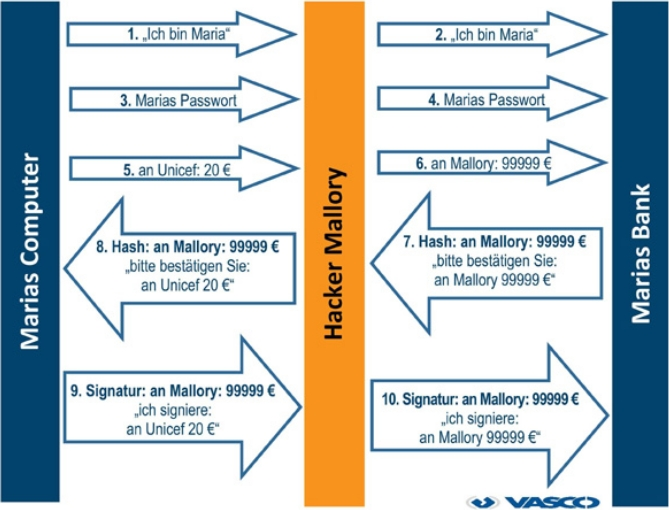
\includegraphics[keepaspectratio=true,height=18\baselineskip]{mitm.jpg}
	\caption{Man in the Middle Attacke}
	\label{fig:rel}
\end{figure}

\subsection{Welche Vorteile hat ein TAN Generator gegenüber einer Streichliste?}
Ein TAN Generator generiert einen one-time Code zur Laufzeit, während dem eine Streichliste beliebig viele Male verwendet werden kann. Somit kann eine Streichliste einfacher gestohlen werden wie ein ein TAN-Generator.

Falls der TAN-Generator zusätzlich zum Code noch weitere Informationen verschickt wie z.B. den Betrag und Empfängername oder -ID, können MITM-Attacken recht wirksam bekämpft werden.

\subsection{Wie könnte eine Phishing-Attacke mittels Pharming und einem Pineapple-Device aussehen?}

\begin{wrapfigure}[13]{R}{0.55\textwidth}
	\centering
	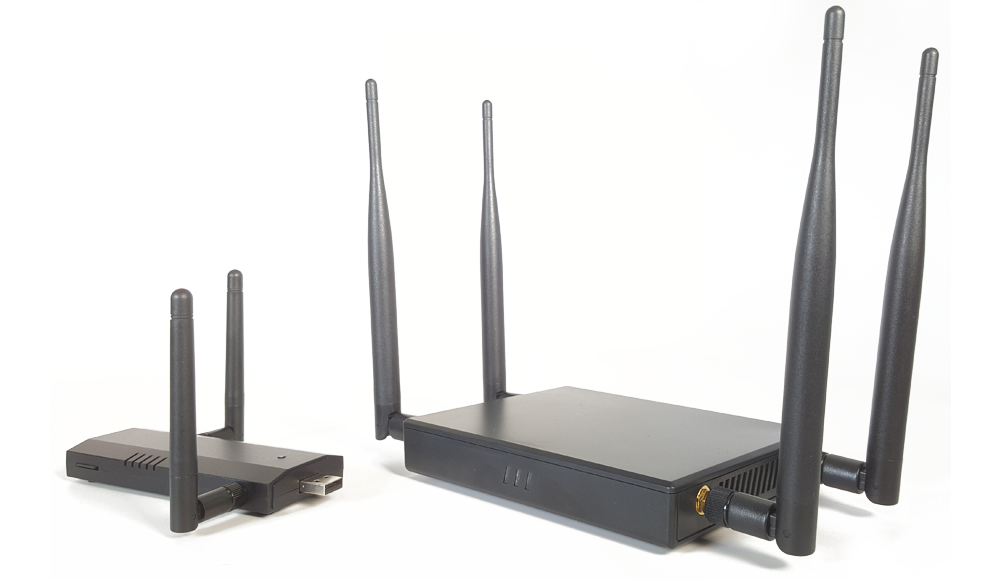
\includegraphics[keepaspectratio=true,height=10\baselineskip]{pineapple.png}
	\caption{WiFi Pineapple Device}
	\label{fig:pineapple}
\end{wrapfigure}

\paragraph{Pineapple Device}\mbox{}\\
Der Wi-Fi Pineapple (Abb. \ref{fig:pineapple}) ist ein Router / WiFi Access Point, der gratis WiFi anbietet, aber für Pentesting / Auditing ausgelegt ist. Er enthält eine Software, die MITM-Attacken ausführen kann, um den Wireless-Verkehr zu sniffen, auditen und manipulieren. 

\paragraph{Pharming}\mbox{}\\
Pharming beschreibt einen Angriff auf DNS-Abfragen. Wenn der Benutzer z.B. e-finance.postfinance.ch aufruft, so erhält er nicht die korrekte IP, sondern die IP einer Phishing-Site.

\vspace{10px}

\noindent Um dies zu erreichen, gibt es verschiedene Methoden:

\begin{description}
	\item [Angriff auf DNS: ] Mittels DNS Spoofing (DNS Cache Poisoning) kann die falsche IP direkt im DNS hinterlegt werden $\rightarrow$ Sehr schwer
	\item [Angriff auf die Host-Datei: ] z.B. Mittels Malware kann direkt im lokalen Hostfile, das vor dem DNS durchsucht wird, einen Verweis von e-finance.postfinance.ch auf die gewünschte IP gemacht werden $\rightarrow$ Bedingt Windows-Betriebssystem
	\item[Netzwerk-Router: ] Es kann im lokalen Netzwerk-Router ein entsprechender Verweis von der Domain auf die gewünschte IP gemacht werden $\rightarrow$ WiFi Pineapple Device ist der Netzwerk-Router, also einfach und plattformunabhängig.
\end{description}

\paragraph{Vorgehen}\mbox{}\\
Man setzt einen sog. "Honey-Pot" auf. Indem man gratis und ungeschütztes Internet anbietet (z.B. mit der SSID "public"), verlockt man Leute dazu auf das Netzwerk zu verbinden. Von nun an geht jede Anfrage die der Benutzer stellt über den Netzwerk-Router (das WiFi-Pineapple), über den ich totale Kontrolle habe. So kann ich, wie bereits erwähnt, jede beliebige Anfrage auf jede beliebige IP umleiten mithilfe des Router-internen DNS'. Der Nutzer merkt davon nichts, ausser er achtet sich auf das SSL-Zertifikat oben links in der Adressliste.

\newpage

\subsection{Erklären Sie SQL Injection Angriffe anhand eines Beispiels}
SQL-Injection bedeutet, dass der Benutzer durch unvalidierte Benutzereingaben Schadcode auf der Datenbank einschleusen ('injecten') kann. Dies geschieht dann, wenn Benutzereingaben ungeprüft direkt in die Datenbank geladen werden.

\paragraph{Beispiel}\mbox{}\\


\begin{lstlisting}[language=php, captionpos=b, caption={PHP Code mit unvalidiertem SQL-Code}]
	<?php
		$sql = "SELECT ID
				FROM USER
				WHERE Benutzer = '".$_POST['Benutzername']."' AND 
						Passwort = '".$_POST['Passwort']."'
				";
		$result = mysql_query($sql);
	?>
\end{lstlisting}

Der oben gezeigte Code ist anfällig für eine einfache SQL-Injection. Ein Benutzer könnten nun als Passwort \verb|'' OR '1' = '1'| eingeben und könnte sich problemlos einloggen. Denn auf PHP-Level würde dieser Loginversuch so aussehen:

\begin{lstlisting}[language=php]
	<?php
		$sql = "SELECT ID
				FROM USER
				WHERE 	Benutzer = 'Admin' AND 
						Passwort = '' OR '1' = '1'
				";
		$result = mysql_query($sql);
	?>
\end{lstlisting}

Somit gibt die Datenbank alle Benutzer zurück, die den Benutzernamen 'Admin' haben. Der Passwort-Check wurde komplett ausgehebelt, da nun gecheckt wird, ob 1 = 1 ist, was immer 'true' zurückgibt.

\vspace{10px}

\noindent Mittles SQL-Injection kann auch fremder Code eingeschmuggelt werden. So könnte man in obenstehenden Szenario auch alle Benutzer löschen, wenn man den String \verb|''; DROP TABLE USER| als Benutzernamen oder Passwort einsetzen würde. Denn ";" zählt als Abschluss eines SQL-Statements. Somit würde man z.B. einen leeren Benutzernamen übergeben und als nächstes, eingeschmuggeltes SQL-Statement die Tabelle 'USER' löschen.

\newpage

\subsection{Mit welchen Methoden können SQL-Injection Angriffe verhindert/erschwert werden?}
Mittels Prepared Statements. Das SQL-Statement wird bereits vordefiniert und die Benutzereingaben werden quasi nur noch als Variablen übergeben.

\begin{lstlisting}[language=php, captionpos=b, caption={Prepared Statement in PHP}]
	<?php
		// Create connection
		$conn = new mysqli($servername, $username, $password, $dbname);
		
		// Check connection
		if ($conn->connect_error) {
		die("Connection failed: " . $conn->connect_error);
		}
		
		// prepare and bind
		$stmt = $conn->prepare("SELECT ID FROM USER WHERE Benutzer=user AND Password=pass) VALUES (?, ?)");
		$stmt->bind_param("ss", $user, $pass);
		
		//set parameters to userinput
		$user = $_POST['Benutzername'];
		$pass = $_POST['Passwort']
		
		//execute statement
		$stmt->execute();
	?>
\end{lstlisting}

\vspace{10px}

\noindent Trotz Prepared Statement, welche SQL-Injection ziemlich ausser Gefecht setzt, sollte kein User-Input unvalidiert zur Datenbank gelangen. Es kann immer noch z.B. mit JavaScript schadhaften Code injiziert werden, der beim nächsten Aufruf der Webiste ausgeführt werden kann.

\section{Teil Portmann}

\section{Teil Bürgler}

\end{document}